\documentclass[tikz,border=10pt]{standalone}
\usetikzlibrary{calc}
\begin{document}
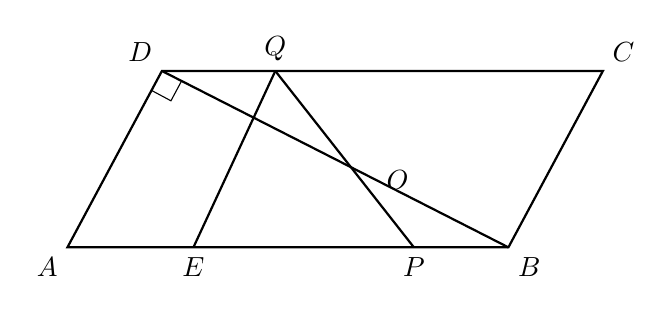
\begin{tikzpicture}[scale=0.8]
\coordinate (A) at (0,0);
\coordinate (B) at (7,0);
\coordinate (C) at (8.5,2.8);
\coordinate (D) at (1.5,2.8);
\coordinate (E) at (2,0);
\coordinate (P) at (5.5,0);
\coordinate (Q) at (3.3,2.8);
\coordinate (O) at ($(D)!0.62!(B)$);
\draw[thick] (A) -- (B) -- (C) -- (D) -- cycle;
\draw[thick] (D) -- (B);
\draw[thick] (E) -- (Q);
\draw[thick] (P) -- (Q);
% right angle mark at D between DA and DB
\draw ($(D)!0.35cm!(A)$) -- ($($(D)!0.35cm!(A)$)!0.35cm!90:(A)$) -- ($(D)!0.35cm!(B)$);
\node[below left] at (A) {$A$};
\node[below right] at (B) {$B$};
\node[above right] at (C) {$C$};
\node[above left] at (D) {$D$};
\node[below] at (E) {$E$};
\node[below] at (P) {$P$};
\node[above] at (Q) {$Q$};
\node[right] at (O) {$O$};
\end{tikzpicture}
\end{document}
